\documentclass[aps,floatfix,superscriptaddress,onecolumn,tightenlines,amsmath,amssymb,nofootinbib,raggedbottom,nobalancelastpage,10pt]{revtex4-2}

\usepackage[utf8]{inputenc}
\usepackage[T1]{fontenc}
\usepackage{braket}
\usepackage{graphicx}
\usepackage{booktabs}
\usepackage{mathtools}	
\usepackage{amssymb}
\usepackage{amsmath}		
\usepackage{amsfonts}
\usepackage{mathrsfs}
\usepackage{color}
\usepackage{amsthm}
\usepackage{psfrag}
\usepackage{ifsym}
\usepackage{dsfont}
\usepackage{enumerate}
\usepackage{enumitem}
\usepackage{multirow} 
\usepackage{lipsum}
\usepackage{float}
\usepackage[separate-uncertainty=true]{siunitx}
\usepackage{setspace}
\usepackage[sort&compress]{natbib}
\usepackage[dvipsnames]{xcolor}


\usepackage{silence}
\WarningFilter{revtex4-1}{Repair the float}

\usepackage{multirow}
\usepackage{booktabs}

\usepackage{hyperref}
\definecolor{refColour}{RGB}{31, 150, 139}
\definecolor{citeColour}{RGB}{68, 1, 84}
\definecolor{extraColour}{RGB}{115,208,85}
\hypersetup{colorlinks=true,linkcolor=refColour,citecolor=citeColour}

\usepackage{titlesec}
\titleformat*{\subsection}{\normalfont\centering}
\titleformat*{\section}{\normalfont\centering\large}

%%%%%%%%%%%%%%%%%%%
%%% newcommands %%%
%%%%%%%%%%%%%%%%%%%

\newcommand{\oos}{\omega_s}
\newcommand{\ooi}{\omega_i}
\newcommand{\oop}{\omega_p}
\newcommand{\ooa}{\left( \oos,\ooi\right)}
\newcommand{\Oos}{\Omega_s}
\newcommand{\Ooi}{\Omega_i}
\newcommand{\Oop}{\Omega_p}
\newcommand{\Ooa}{\left( \Oos,\Ooi\right)}
\newcommand{\dg}{^{\dagger}}

\newcommand*\hgzero{\includegraphics[height=7pt]{hg0.pdf}}
\newcommand*\hgone{\includegraphics[height=7pt]{hg1.pdf}}

\renewcommand{\figurename}{Figure}
\renewcommand{\tablename}{Table}

\newcommand{\ketbra}[1]{ | #1 \rangle\!\langle #1 |}
\newcommand{\iketbra}[1]{ | #1 \rangle\!_{_i}\langle #1 |_{_i}}
\newcommand{\sketbra}[1]{ | #1 \rangle\!_{_s}\langle #1 |_{_s}}

\newcommand{\der}[2] {\frac{d #1}{d #2}}
\newcommand{\dersq}[2] {\frac{d^2#1}{d #2^2}}
\newcommand{\parder}[2] {\frac{\partial #1}{\partial #2}}
\newcommand{\parderst}[2] {\frac{\partial #1}{\partial #2}}
\newcommand{\pardersq}[2] {\frac{\partial^2}{\partial #2^2} #1}
\newcommand{\pardersqst}[2] {\frac{\partial^2 #1}{\partial #2^2}}
\newcommand{\pibar} [0] {\: \: \makebox[0pt]{$\pi$} \raisebox{-0.8ex}{$\bar{}$}}
\newcommand{\inbg} [0] {\: \: \makebox[0pt]{!}\hspace{-0.5 ex}{?}}
\newcommand{\ldiagpol} [0] {\: \: \makebox[0pt]{$\nwarrow$}\hspace{-1.1 ex}{\searrow}}
\newcommand{\rdiagpol} [0] {\: \: \makebox[0pt]{$\nearrow$}\hspace{-1.2 ex}{\swarrow}}
\newcommand{\tb} [1] {\textbf{#1}}
\newcommand{\mr} [1] {\mathrm{#1}}
\newcommand{\vs} [2] {\textbf{#1}_{\mathrm{#2}}}
\newcommand{\vc} [2] {\textbf{#1}_{#2}}
\newcommand{\cat} [3] {\ket{#1}{#3}{#2}\ket{{-}#1}{#3}}
\newcommand{\sqo} [1] {\hat{S}_r\ket{1}{#1}}
\newcommand{\sqot} [2] {\hat{S}_{#2}\ket{1}{#1}}
\newcommand{\sqov}[2] {\hat{S}_{#2}\ket{0}{#1}}
\newcommand{\ii} {\textbf{i}}
\newcommand{\ve} {\varepsilon}
\newcommand{\Tr} {\operatorname{Tr}}

\newcommand{\expec}[1]{\left\langle #1 \right\rangle}
\newcommand{\one}{\leavevmode\hbox{\small1\normalsize\kern-.33em1}}
\newcommand{\sandwich}[3]{\mbox{$ \langle #1 | #2 | #3 \rangle $}}

\newcommand{\dket}[1]{\mbox{$\left|\left.#1\right\rangle\right\rangle$}}
\newcommand{\dbra}[1]{\mbox{$\left\langle\left\langle #1\right.\right|$}}
\newcommand{\dbradket}[2]{\mbox{$\langle\langle #1|#2\rangle\rangle$}}
\newcommand{\dketdbra}[2]{\mbox{$|#1\rangle\rangle\langle\langle #2|$}}

\newcommand{\dbraket}[2]{\mbox{$\langle\langle #1|#2\rangle$}}
\newcommand{\dketbra}[2]{\mbox{$|#1\rangle\rangle\langle #2|$}}
\newcommand{\bradket}[2]{\mbox{$\langle\ #1|#2\rangle\rangle$}}
\newcommand{\ketdbra}[2]{\mbox{$|#1\rangle\langle\langle #2|$}}

\newcommand{\id}{\mathds{1}}
\newcommand{\Ident} {\mathds 1}
\DeclareMathOperator{\tr}{tr}
\newcommand{\mm}{{\cal M}}

\newcommand{\changed}[1]{\textcolor{red}{ #1}}
\newcommand{\todo}[1]{\textbf{\textcolor{blue}{ #1}}}
\newcommand{\reply}[1]{\textcolor{magenta}{ #1}}
\newcommand{\new}[1]{\textcolor{cyan}{ #1}}
\newcommand{\change}[1]{\textcolor{blue}{ #1}}
\newcommand{\alex}[1]{\textit{\small\bfseries\textcolor{black}{AP: #1}}}

\begin{document}

\title{\normalfont\Large{Towards an 8 Photon Graph}}
\maketitle

%\section*{Computing $\gamma$ Parameter} 
%
%In order to gain knowledge of the squeezing parameter we need singles and coincidences of the non-linear source as a function of the pump power. The probability that the non-linear photon source produces n photons is given by,
%
%\begin{align}\label{eq:geoDist}
%    (1 - P \tau ) (P \tau )^n = (1 - \gamma^{2})(\gamma^2)^n.
%\end{align}
%
%Where $\tau$ defines the interaction within the media given a pump power of $P$. Expressed with respect to $\gamma$, $\gamma = \sqrt{p \tau}$. The $\gamma$ parameters importance is evident when you express the down-conversion process as a series expansion of photon number terms in signal and idler modes:
%
%\begin{align}
%    \ket{\psi}_{\text{\tiny{PDC}}} &= \sqrt{1 - \gamma^2} \sum^{\infty}_{n=0} \gamma^n \ket{n,n} \\
%     &= \sqrt{1-\gamma^2} \hspace{.5em} (\ket{0,0} + \gamma \ket{1,1} + \gamma^2\ket{2,2} + \hspace{.5em}  ... \hspace{.5em} ).
%\end{align}
%
%The parameter $\gamma$ now dictates the probability of photon pair emission, i.e $\gamma^n(1-\gamma^2)$ is the probability of n-pairs of photons being generated. Typically we seek $n=1$ from the same pump pulse in two separate crystals. However, due to probabilistic nature of these photon sources, having two independent sources producing $n=1$ pairs of photons is the equivalent probabilistically as having a single source producing $n=2$ pairs. We use a geometric distribution to represent photon number statistics from pulsed source as we stated in Equation (\ref{eq:geoDist}), where the probability of n-fold emission is,
%
%\begin{equation}
%    p_{\text{em}}(P,n,\tau) = (1 - P \tau)(P \tau)^n 
%\end{equation}
%
%We deploy SNSPD's to detect the arrival of a photon. These are non-number resolving detectors which simply click when $n>0$ photons arrive. If we are considering that there are n photons generated, we may only be capable of detecting k out of n photons due to the operational nature of the SNSPD's. The detection probability of detecting at least k photons given n photons in a single mode is therefore:
%
%\begin{equation}
%  p_{\text{det}}(\eta,n,k) = 1 - \sum_{m=0}^{k-1} \binom{n}{k} \eta^m (1-\eta)^{n-m}
%\end{equation}
%
%An additional function which adds extra accuracy in representing the final photon number statistics of our system is the probability that the detectors, which have an associated dead-time after a detection event, are ready to detect photons again. The probability that a detector is ready is the probability that firstly, photons are emitted from the source combined secondly, with the probability that within a time window $t$--equivalent to the dead-time associated with that detector--no photon was detected. This is written as, 
%
%\begin{equation}
%    p_{\text{ready}}(P,R,t,\tau,\eta_1,\eta_2) = \big[ \sum^{\infty}_{i=0} p_{\text{em}}(P,i,\tau) \cdot p_{\text{det}}(1-\eta_1,i,i) \cdot p_{\text{det}}(1-\eta_2,i,i) \big]^{\lfloor R\times t \rfloor},
%\end{equation}
%
%where $R$ is the repetition rate of our pump in Hz, $t$ is the detectors dead-time, and the exponent is wrapped in a floor function which rounds to the nearest integer less or equivalent to the value the function is being applied to. With these three functions we can now begin to build a model which approximates the photon rates we expect to see post detection. For the rates of single photon detection the function reads as,
%
%\begin{equation}
%    R_s(P,R,t,\tau,\eta) = R \Big(\big[ \sum^{\infty}_{j=1}  p_{\text{em}}(P,j,\tau) \cdot p_{\text{det}}(\eta,j,1) \big] p_{\text{ready}}(P,R,t,\tau,\eta,0) \Big).
%\end{equation}
%
%For multi-photon experiments we are interested in rates of coincidences from $N$-photon sources, the probability of such events are,
%
%\begin{equation}
%    R_{cc}(P,R,t,\tau,\eta_{m_1},\eta_{m_2},N) = R \cdot \prod_{m=1}^{N} \Big(p_{\text{em}}(P,j,\tau_m) \cdot p_{\text{det}}(\eta_{m_1},1,1) \cdot p_{\text{det}}(\eta_{m_2},1,1) \cdot  p_{\text{ready}}(P,R,t,\tau_m,\eta_{m_1},\eta_{m_2}) \Big).
%\end{equation}\label{eq:generationRates}
%
%Using these functions we can extract the parameters $\tau$, $\eta_1$ and $\eta_2$ for each source. This is achieved by minimising the following:
%
%\begin{equation}
%    \mid \text{Singles}_1(P) - R_s(P,t,\tau,\eta_1) \mid + \mid \text{Singles}_2(P) - R_s(P,t,\tau,\eta_2) \mid + \mid \text{Coincidences}(P) - R_{cc}(P,t,\tau,\eta_1,\eta_2) \mid,
%\end{equation}
%
%given that we know the single and coincidence rates as a function of power, we know the repetition rate and detector dead-times, we can obtain numerical values for $\tau$, $\eta_1$ and $\eta_2$. These values can then be used inside Equation \ref{eq:generationRates} to output the expected rates from N sources.

\section*{Expected Rates From Sagnac Sources} 

In the case of most previous results obtained via the above method we always had the photon source configured such that a separable state was produced. Although this is fine to use for the analysis in the Gaussian crystal paper--where we only consider that the source is set up in such a way--when it comes to approximating the rates we would see for an 8 photon GHZ state, the sources will be producing Bell states. In this configuration one cannot assume that we can achieve the same brightness and efficiencies that we achieved with the pair source due to the greater complexity in optical alignment. Therefore, a better understanding of source performance is to align the sources in a way that produces Bell pairs, and run a power dependence, performing tomography at these powers and then gathering the singles and coincidences from these measurements. 

%At this point it is important to state that, when this data was taken, the tomography stage was lossy. Compared to straight to the detectors, the tomography stage introduced a 30\% reduction to the coincidence counts. This reduction was checked and was a result of coupling, general optical loss from surfaces and the combination of extinction ratio and non-ideal polarisation incident on the PBS. All of the things we could address have now been addressed with the 1550 diode. The characterisation of losses with details are in the OneNote page when we come round to making any improvements.

%\begin{figure}[ht] \vspace{2em}
%    \begin{center}
%    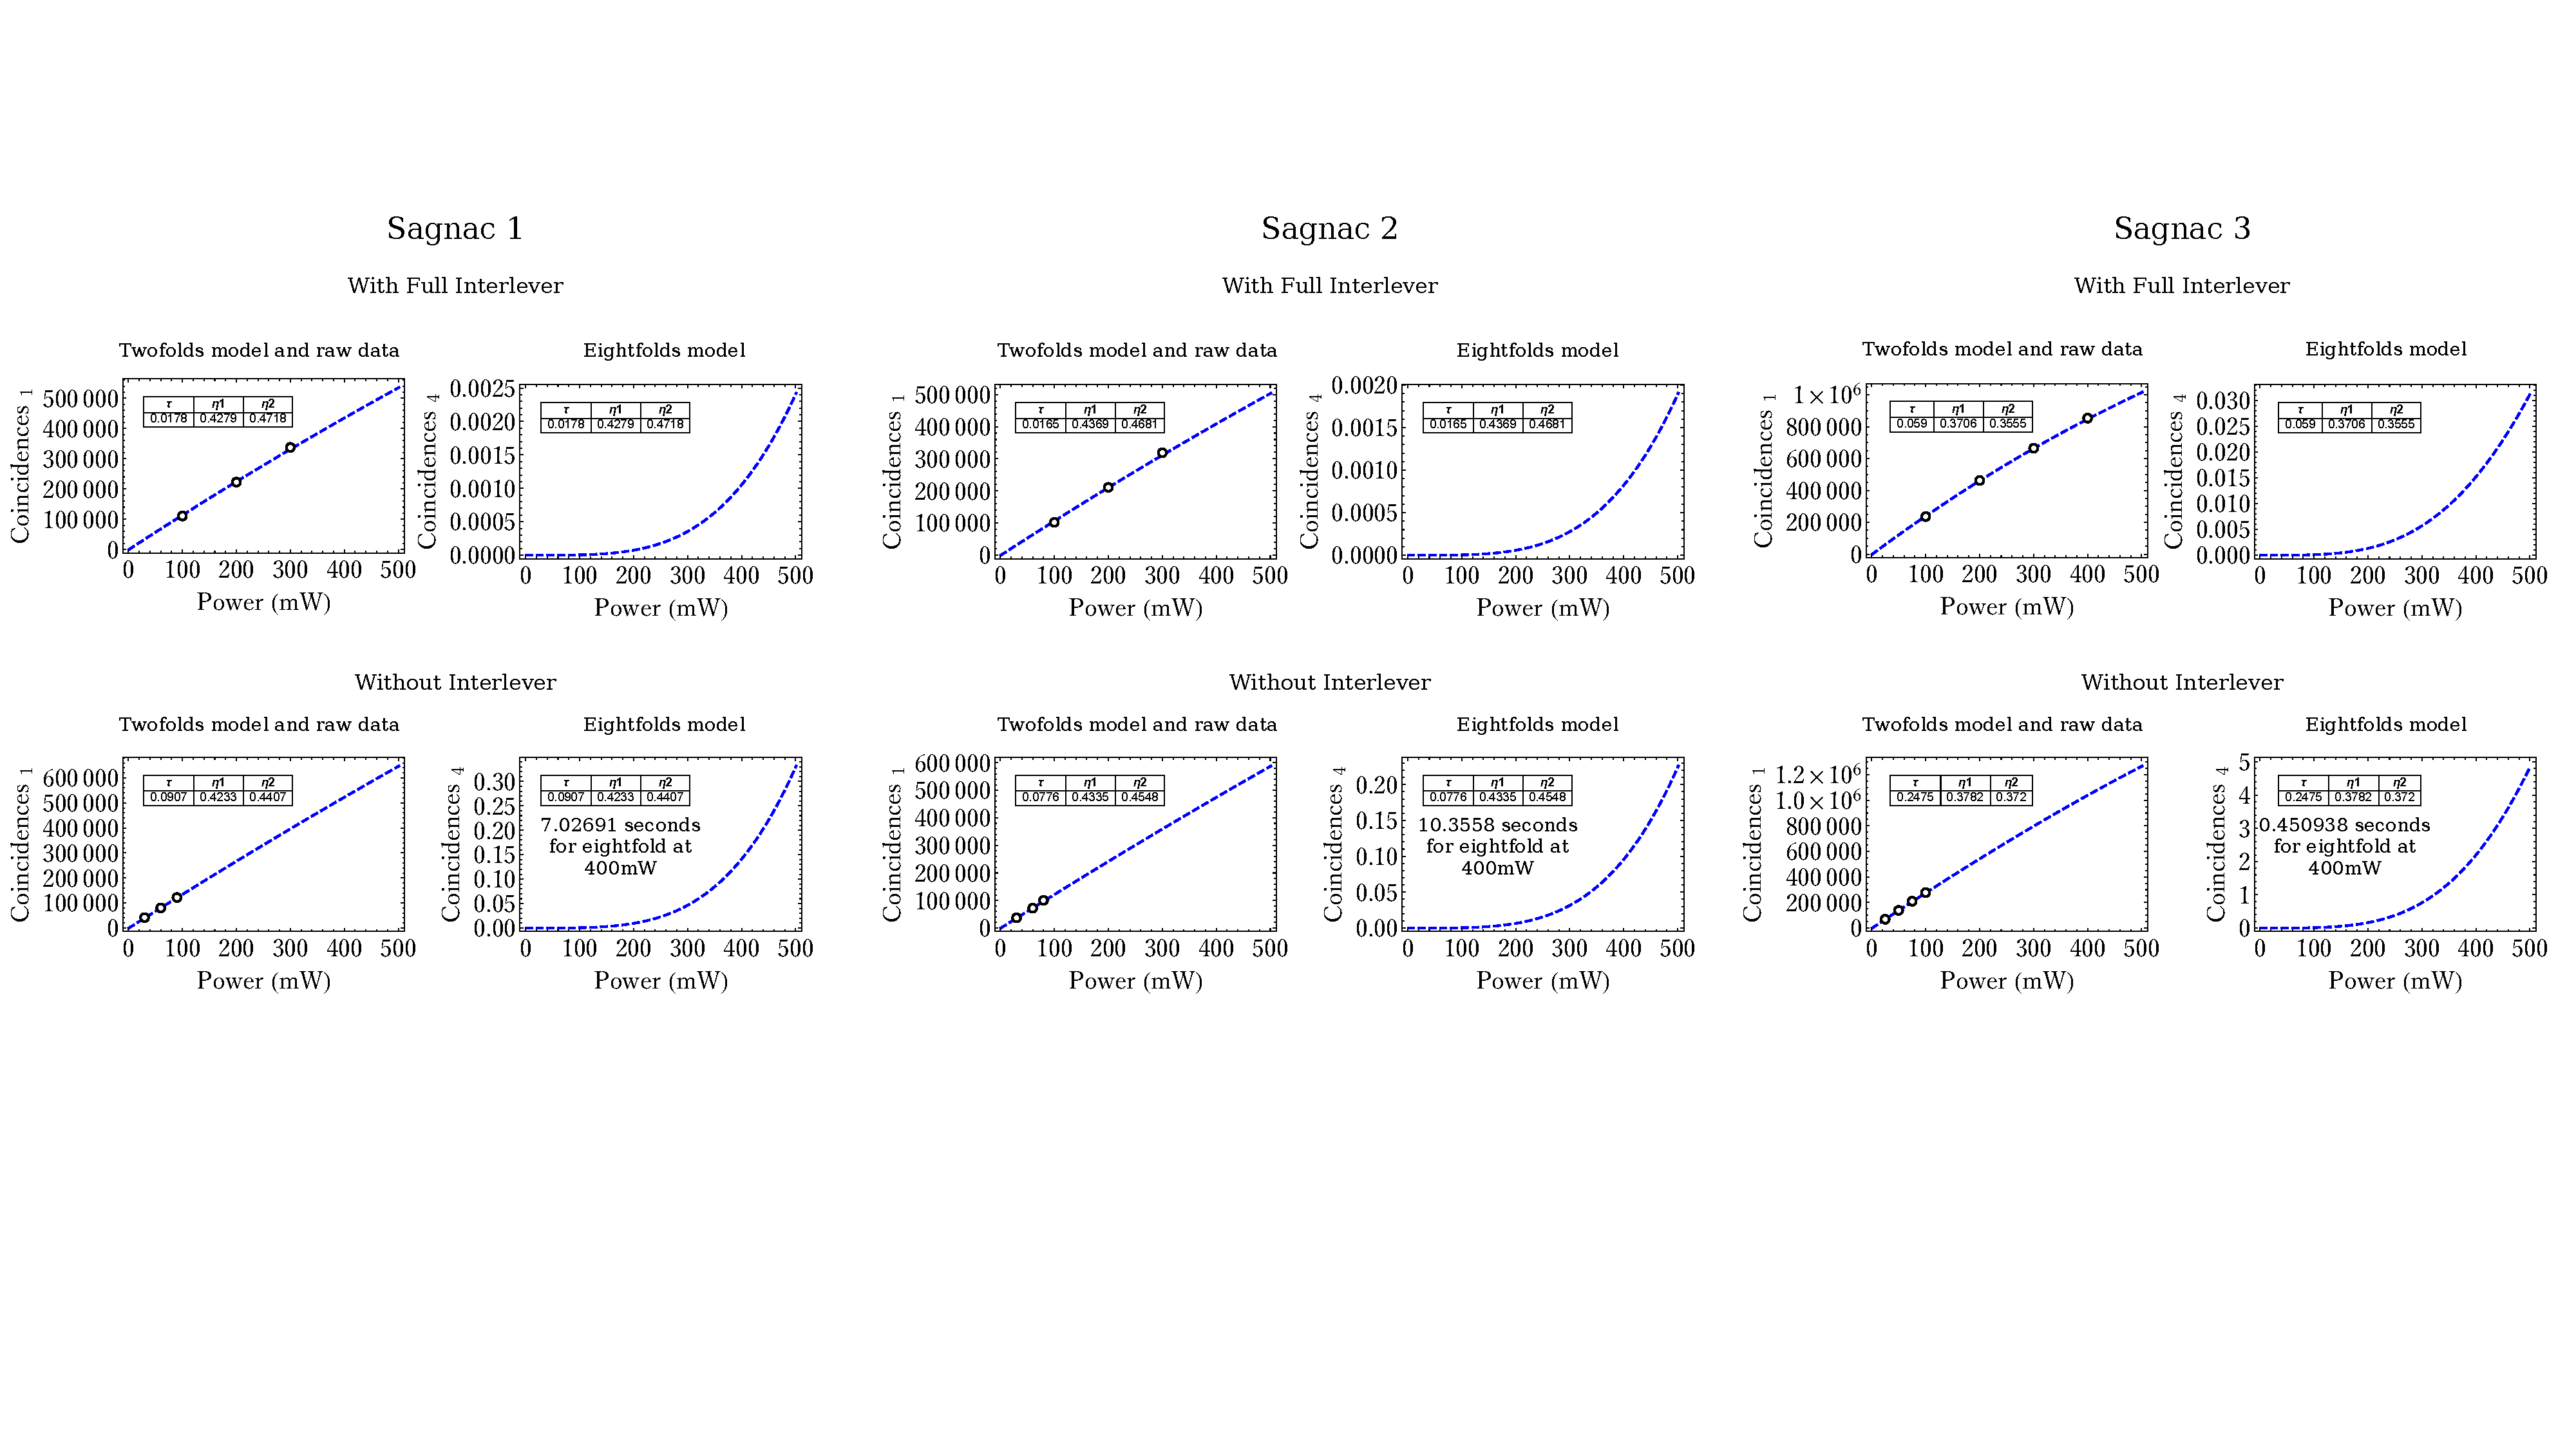
\includegraphics[width=\textwidth]{figures_detectorModel/exp_detectorModelFigures.pdf}
%    \end{center}\vspace{-2em}
% 
%    \caption{\textbf{Sagnac 1} containing aKTP with a 50cm focusing lens and 20cm collection distance. \textbf{Sagnac 2}  also containing aKTP with a 50cm focusing lens and 20cm collection distance. Then \textbf{Sagnac 3} contains ppKTP filtered with Alluxa filters with a 40cm focusing lens and 20cm collection distance. All of the rate outcomes have not been adjusted to what an 8 fold GHZ state would be, so the times should be multiplied by $(\textsf{vis}(1/2))^{3}$ for the success rates of three fusion gates given an interference visibility \textsf{vis}.}
%    
%\end{figure}

\section*{Crude Calculation of Rates} 

Rather than relying on the model, we can use the following function to quickly work out what rate we would expect with known brightness,  pump power, repetition rate and interference visibility:

 \begin{equation}
	(\frac{\text{Brightness}\times\text{Power}}{\text{Repetition Rate}})^{4} \times \text{Repetition Rate} \times (\text{Visibility} \times \frac{1}{2})^{3}.
\end{equation}

Now, we can use this function to estimate the expected maximum 8-fold rate for a GHZ state involving three fusions. For the "Experimental Ten Photon Entanglement" JWP paper they quoted an 8 photon GHZ state rate of 0.2Hz. Using the crude calculation with 85\% visibility and an overall throughput of 90\%, the function outputs 0.1908Hz, roughly the quoted rate. For our sources, assuming 89.8\% and 83.3\% interference visibility for aKTP (with semrocks) and ppKTP respectively (calculated from the interference experiments pre-lockdown, where the results are in the gaussian paper and extrapolating the linear fit), and the brightnesses we could achieve with a 40cm focus lens of 3.6kHz (only seen in a non-collinear operation) and 4kHz, the rates for our crystals are 0.39Hz and 0.48Hz. Thats around double the rates of JWP. We could then potentially afford to use one pass of the interlever for gains in state purity and fidelity. These rates would then need to be scaled by a factor of 8 to 0.07 and 0.08 respectively for aKTP and ppKTP.

\section*{Moving Towards 400mW of Pump Power} 

Some things to consider are; whether the linear extrapolation is an okay treatment, we would need to run this test when we can achieve at least 400mW in each Sagnac. We should also investigate how accurately we can overlap any arms of a "smaller" interlever. The plan discussed so far is to not have a "long" arm to put the successive pulses symmetrically between each other, but to use a shorter arm that is designed to up the repetition rate whilst enabling an easier and more stable overlap.

%\begin{figure}[ht] \vspace{2em}
%    \begin{center}
%    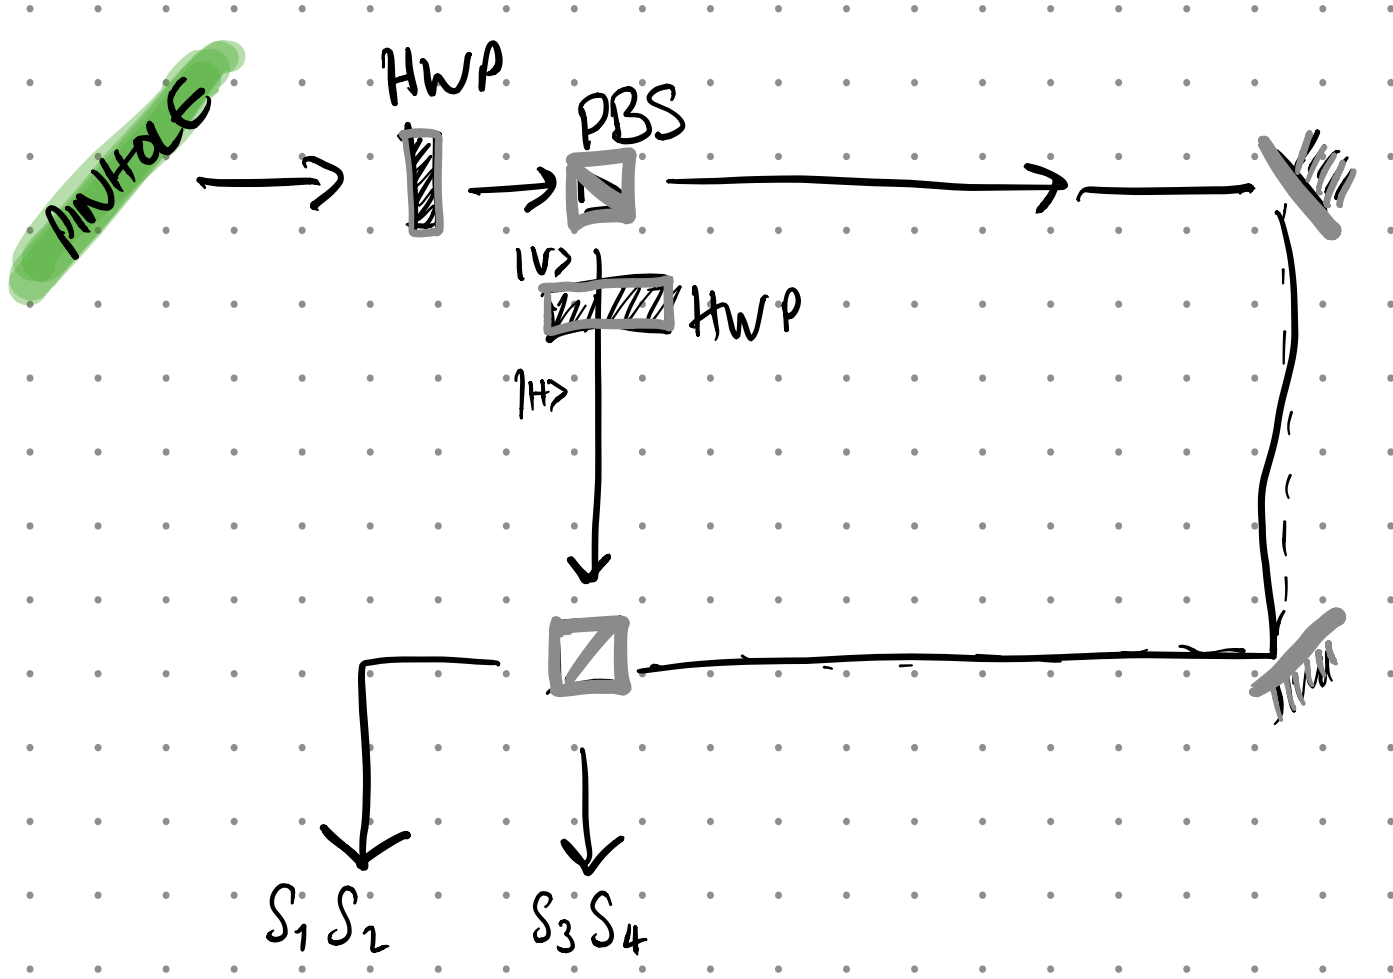
\includegraphics[width=4cm]{figures_detectorModel/int.png}
%    \end{center}\vspace{-1em}    
%    
%      \caption{We could not build a four pass interlever in this fashion but as we will be looking at just having one arm to interleve pulses, we can use the HWP and PBS combination to transition between 80MHz and 160Mhz repetition rates.}
%    
%\end{figure}

\section*{Lens Configurations} 

From the the detector model results it is clear to see that we need shorter focal length lenses (I would say that 40cm is a minimum) to achieve the rates we desire. At the moment we have 40cm lens and 50cm lens available for S3, S4 and S1, S2 respectively. We however need to prioritise getting the highest brightness we can. This means that we should be using 40cm lenses or shorter. There is a limit to how short a lens we can use and this limit is bound by two things: the placement of the BS's that separate the pump into two sources and the distance from the crystal to the coupling lenses. However, from a previous scan of distance from crystal to couplers using a Sagnac we can get to 20cm collection distances.

\vspace{1em}  

Interestingly, we could get up to 8kHz with ppKTP and 6kHz brightness with aKTP (with semrocks) within the limits of allowable collection distances. But placing a 25cm focusing lens in front of the Sagnacs is something that may not be achievable. Seeing as we are going to be altering the interlever, maybe being able to focus with 25cm, or somewhere between 25cm and 40cm lenses into the Sagnacs is something we should consider. 

\begin{figure}[h] \vspace{2em}
    \begin{center}
    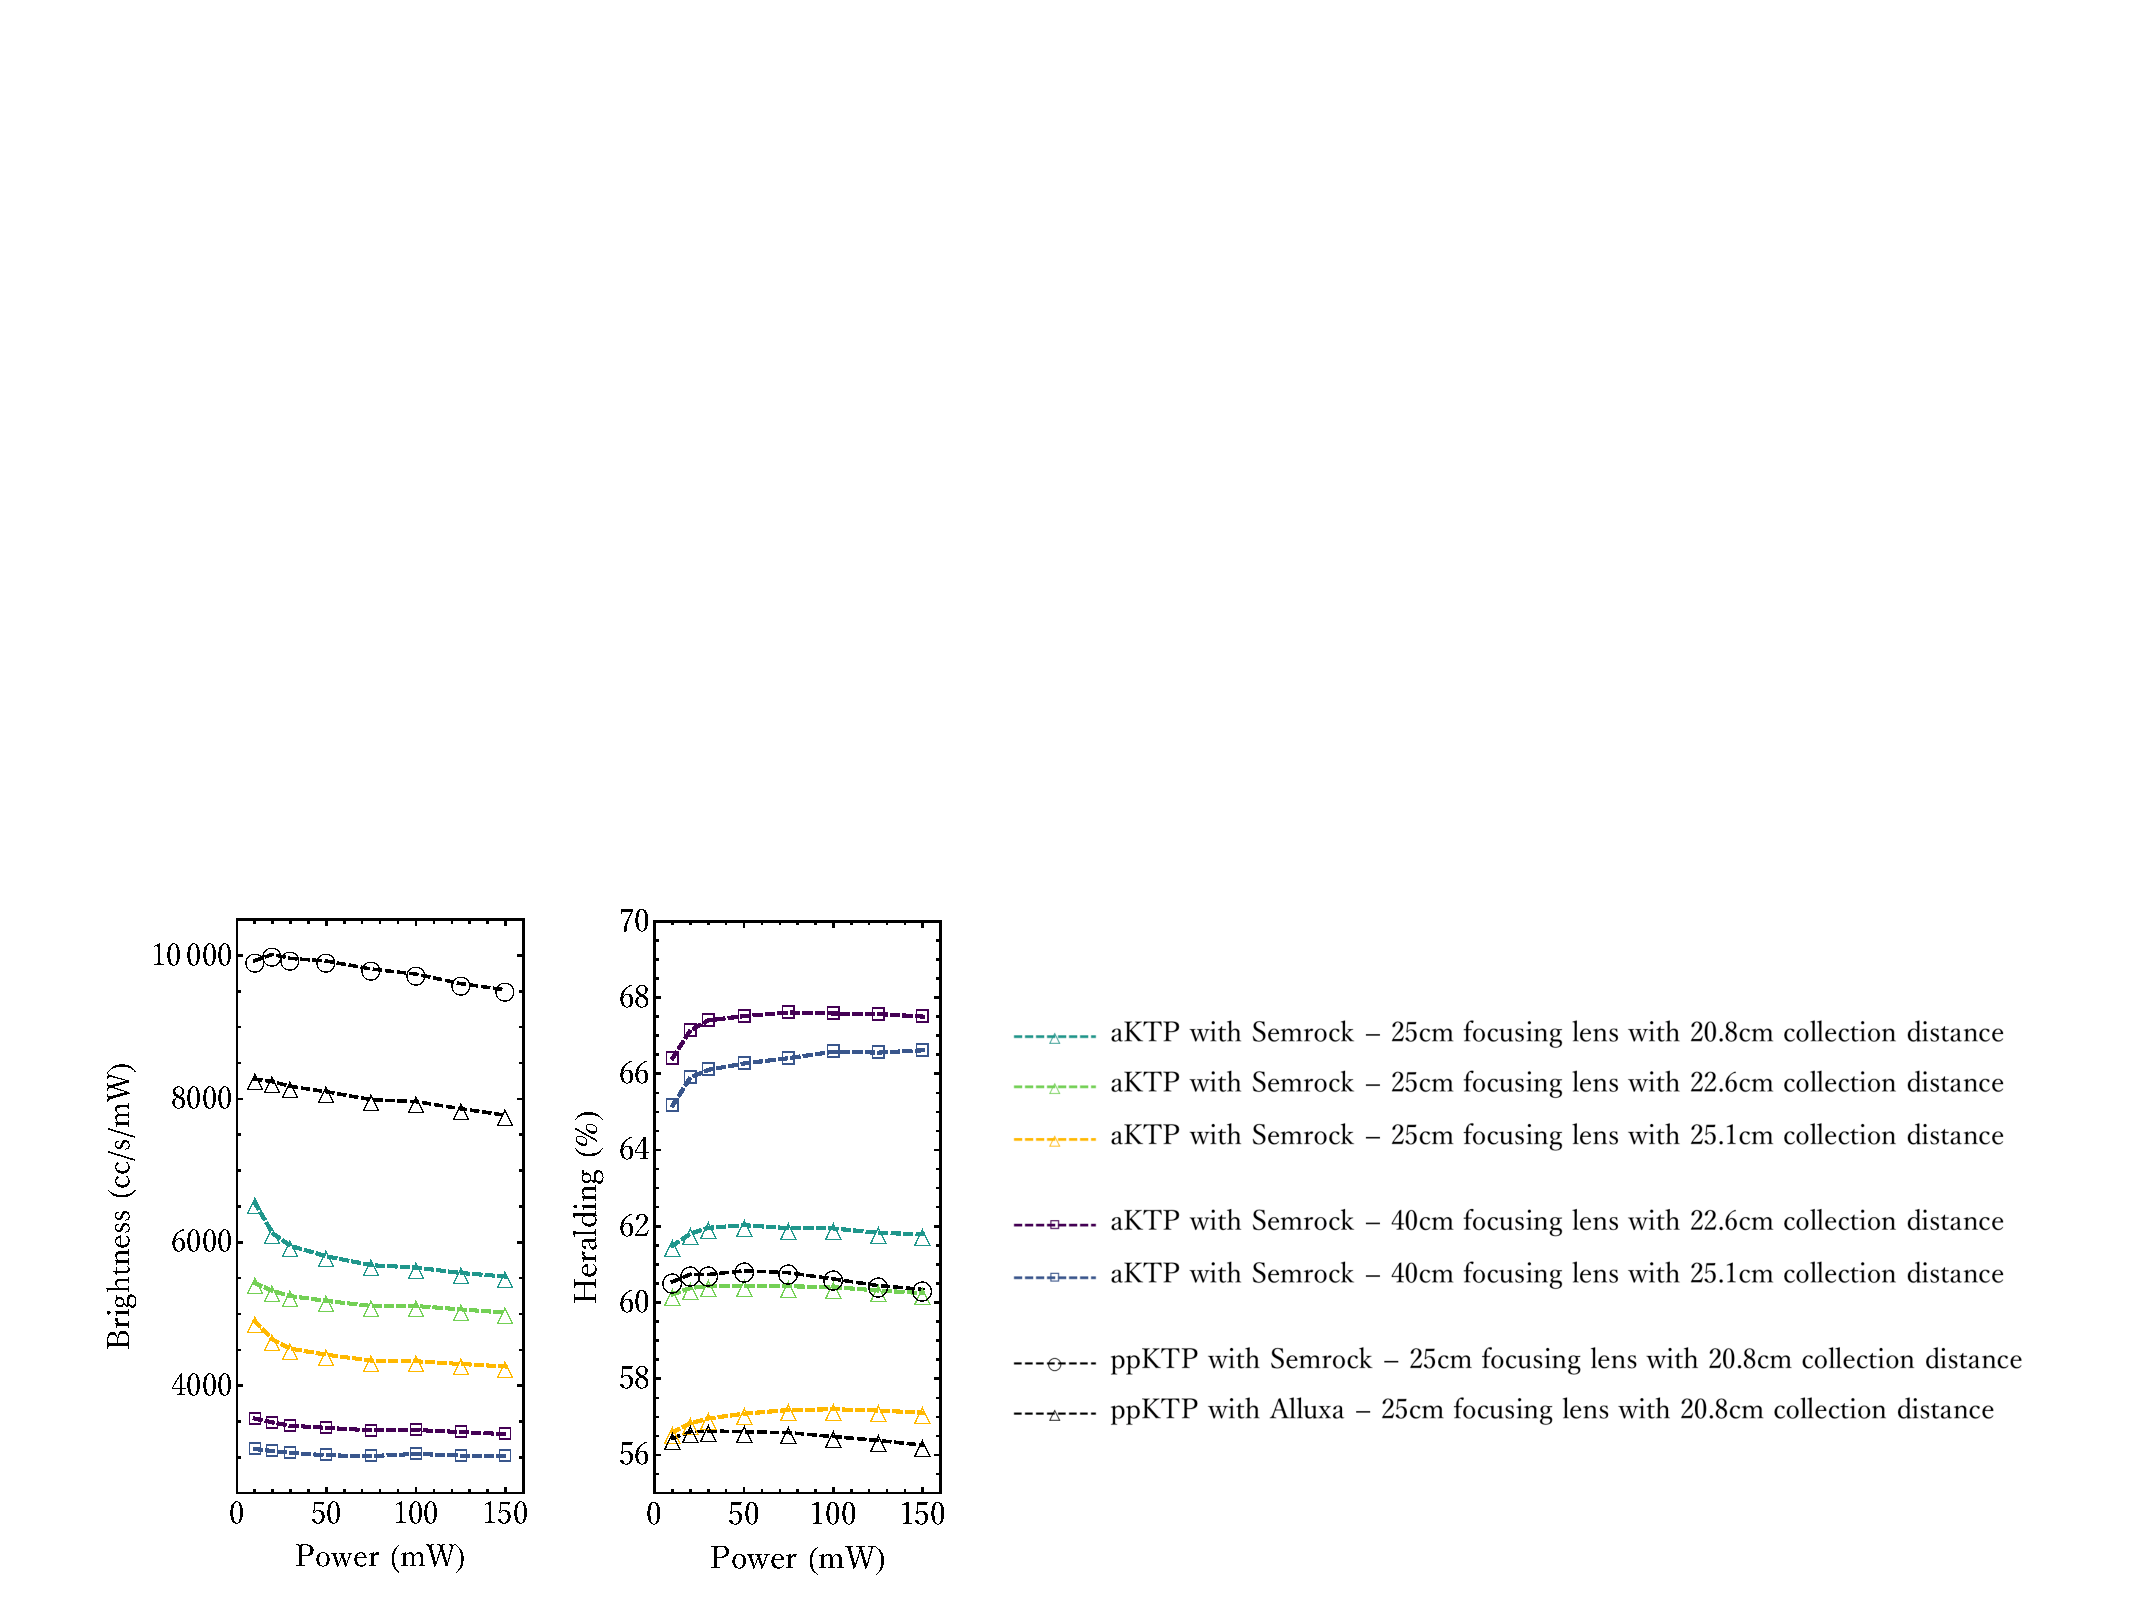
\includegraphics[width=16cm]{figures_detectorModel/heraldingBrightnessFocus.pdf}
    \end{center}\vspace{-1em}    
\end{figure}

\section*{Novelty} 

We should be more than capable of achieving better rates than JWP, given the brightnesses we have seen and according to the crude model, but something that adds a large degree of novelty to this work would be to remove all spectral filtering (other than silicon windows to block the pump). This is convenient as it also means we will not have to order another 4 semrock filters whilst we exploit the new aKTP's ability to allow these multi-photon experiments without filtering. The actual coincident count rate should differ by (some percentage I will work out) with the caveat of a drop in interference visibility of 3.7\% (at 400mW of pump power). 

\vspace{1em}

So far, without filtering, we have seen 3600cc/mW (with good colineararity in the sagnac) which, using the crude model, gives an 8-fold rate of $\sim$0.35 Hz. This rate represents an upper bound based on 10\% loss (same as JWP quoted) and the relevant losses applied to fusions that depend on the interference visibility of aKTP without filters at 400mW of pump power. With shorter lenses we could gain significantly more rates. A shorter lens with aKTP could potentially produce a brightness of  $\sim$5000cc/mW. Then the eightfold rate is 1.3Hz. If we deployed the interlever with this brightness, we could achieve a rate of 0.16Hz, comparable to JWP rates but with, in theory, a higher quality state. 

\vspace{1em}

The next steps will be to build the new interlever, decide on a lens configuration, and run independent HOM between two sources,. This will let us obtain the 4 fold rates that can be mapped to the detector model outputs. That then should further help us predict a more realistic 8 photon rate.

\end{document}

































































